\documentclass[tikz,border=3pt]{standalone}
\usepackage[utf8]{inputenc}
\usepackage{pgfplots}
\pgfplotsset{compat=1.18}

\definecolor{decreaseblue}{HTML}{0072B2}
\definecolor{samegray}{HTML}{9CA3AF}
\definecolor{increaseorange}{HTML}{D55E00}

\begin{document}
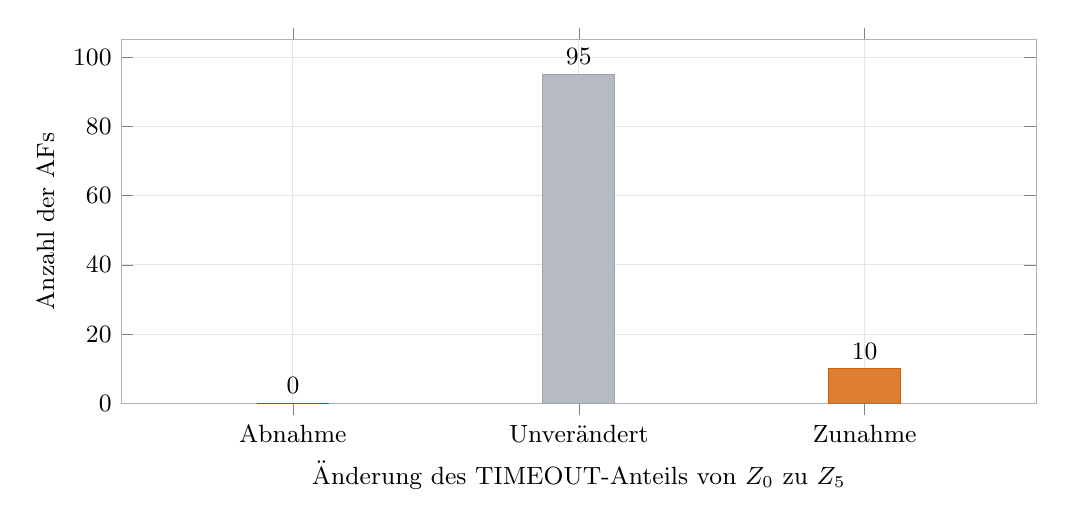
\begin{tikzpicture}
\begin{axis}[
    width=13.2cm,
    height=6.2cm,
    ybar,
    bar width=26pt,
    ymin=0,
    ymax=105,
    ytick={0,20,40,60,80,100},
    symbolic x coords={Abnahme,Unverändert,Zunahme},
    xtick={Abnahme,Unverändert,Zunahme},
    xlabel={Änderung des TIMEOUT-Anteils von $Z_0$ zu $Z_5$},
    ylabel={Anzahl der AFs},
    grid=major,
    grid style={draw=gray!20},
    axis line style={draw=gray!60},
    tick label style={font=\small},
    label style={font=\small},
    nodes near coords,
    every node near coord/.append style={font=\small,anchor=south,text=black},
    enlarge x limits=0.30
]
\addplot+[bar shift=0pt,draw=decreaseblue,fill=decreaseblue!75] coordinates {(Abnahme,0)};
\addplot+[bar shift=0pt,draw=samegray,fill=samegray!75] coordinates {(Unverändert,95)};
\addplot+[bar shift=0pt,draw=increaseorange,fill=increaseorange!80] coordinates {(Zunahme,10)};
\end{axis}
\end{tikzpicture}
\end{document}
